% TEMPLATE for Usenix papers, specifically to meet requirements of
%  USENIX '05
% originally a template for producing IEEE-format articles using LaTeX.
%   written by Matthew Ward, CS Department, Worcester Polytechnic Institute.
% adapted by David Beazley for his excellent SWIG paper in Proceedings,
%   Tcl 96
% turned into a smartass generic template by De Clarke, with thanks to
%   both the above pioneers
% use at your own risk.  Complaints to /dev/null.
% make it two column with no page numbering, default is 10 point

% Munged by Fred Douglis <douglis@research.att.com> 10/97 to separate
% the .sty file from the LaTeX source template, so that people can
% more easily include the .sty file into an existing document.  Also
% changed to more closely follow the style guidelines as represented
% by the Word sample file. 

% Note that since 2010, USENIX does not require endnotes. If you want
% foot of page notes, don't include the endnotes package in the 
% usepackage command, below.

% This version uses the latex2e styles, not the very ancient 2.09 stuff.
\newcommand{\cks}[1]{\emph{cks: #1}}
\newcommand{\comment}[1]{}

\documentclass[letterpaper,twocolumn,10pt]{article}
\usepackage{graphicx}
\usepackage{usenix,epsfig}
\usepackage{url}
\usepackage{listings}
\usepackage{subfigure}
\usepackage{paralist}
%\usepackage[compact]{titlesec}
%\titlespacing{\section}{0pt}{2ex}{2ex}
%\titlespacing{\subsection}{0pt}{1ex}{1ex}
%\titlespacing{\subsubsection}{0pt}{0.5ex}{0ex}

\begin{document}

%don't want date printed
\date{}

\title{\Large \bf Security Audit of Safeplug ``Tor in a Box''}
\author{
 {\rm Anne Edmundson}\\
 Princeton University\\
 annee@cs.princeton.edu
 \and
 {\rm Anna Kornfeld Simpson}\\
 Princeton University\\
 aksimpso@cs.princeton.edu
 \and
 {\rm Joshua A. Kroll}\\
 Princeton University\\
 kroll@cs.princeton.edu
 \and
 {\rm Edward W. Felten}\\
 Princeton University\\
 felten@cs.princeton.edu
} % end author

\maketitle

%\thispagestyle{empty}

\subsection*{Abstract}
We present the first public third-party security audit of Pogoplug's Safeplug device, which markets ``complete security and anonymity online'' by using Tor technology to protect users' IP addresses.  We examine the hardware, software, and network behavior of the Safeplug device, as well as the user experience in comparison to other forms of web browsing.  Although the Safeplug appears to use Tor as advertised, users may still be identified in ways they may not expect.  Furthermore, an engineering vulnerability in how the Safeplug accepts settings changes would allow an adversary internal or external to a user's home network to silently disable Tor or modify other Safeplug settings, which completely invalidates the security claims of the device.  Beyond this problem, the user experience challenges of this type of device make it inferior to the existing gold standard for anonymous browsing: the Tor Browser Bundle.

%\setlength{\parskip}{1ex plus 2ex minus 2ex}

\section{Introduction}
Privacy on the Internet is becoming increasingly important as users realize how vulnerable they are to tracking, surveillance, and theft of their data.  A recent Pew study listed compromised emails/accounts, harassment, stolen Social Security Numbers, bank information, and credit card numbers as some of the results of online visibility; according to the study, 86\% of Internet users have tried to become more anonymous online~\cite{pew}.  Despite this, users do not believe that they have the tools to solve this problem.

In December 2013, the cloud storage company Pogoplug released the Safeplug, a small box that plugs into a user's home router.  It claims to: conceal your identity, hide where you live, shield your surfing habits, and make you anonymous online by routing all traffic through Tor~\cite{safeplug}.  We conducted the first public third-party security audit of the Safeplug by analyzing the hardware, software, network behavior, and usability of the device.  The following are some of our findings:

\begin{compactitem} \setlength{\itemsep}{.2mm}
\item The Safeplug functions as a HTTP proxy for the browser, which then uses Tor for outgoing traffic.
\item Despite the use of Privoxy as an ad-blocker, the Safeplug does nothing to prevent users' browsers from collecting both first- and third-party tracking cookies, allowing users to be de-anonymized across websites despite the presence of Tor~\cite{arvindpets}.
\item Safeplug users are vulnerable to a Cross-Site Request Forgery (CSRF) attack that allows an attacker external to their home network to modify the Safeplug settings (including silently turning off the use of Tor).
\item A malicious user within the network can modify the Safeplug settings without notifying any other devices on the network.
\item The Safeplug has a higher web request latency than that of the Tor Browser Bundle.
\item The use of the Safeplug provides less protection than the use of the Tor Browser Bundle.
\end{compactitem} 

Pogoplug made use of good security principles by using auditable open source software on their device, and has the laudable goal of making online security the standard for more users. However, there are other technologies available that aim to provide the same functionality, such as the Tor Browser Bundle, which can be used free of charge.  In order to determine if the Safeplug provides value to users, we measure the privacy implications between the different technologies.  We show that there is little reason to use the Safeplug over the Tor Browser Bundle; in addition to the Tor network technology used in the Safeplug, the Tor Browser Bundle contains protections against tracking cookies and fingerprinting, making it an improvement over the privacy offerings of the Safeplug.

%\begin{figure}
%\centering
%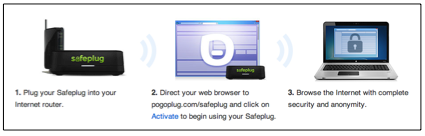
\includegraphics[width=.45\textwidth]{instructions2}
%\caption{Setup instructions (and the only documentation) that came in the box with the Safeplug. Pogoplug highlights the ease of installing the device but does not give a clear indication of how the Safeplug functions.}
%\label{fig:instructions}
%\end{figure}  

%\begin{figure*}
%\centering
%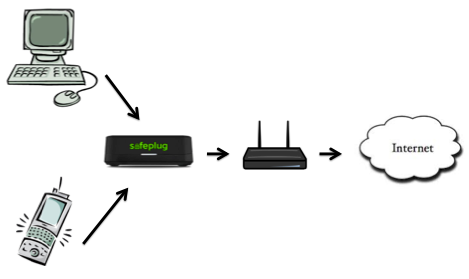
\includegraphics[width=.4\textwidth]{safeplug_flowchart}
%\caption{Flowchart demonstrating the actual functionality of the Safeplug as an HTTP proxy between a device's browser and the home network's router.}
%\label{fig:flow}
%\end{figure*} 

%\section{Background}
%Safeplug \cite{safeplug}, is a product that launched in December of 2013 from the cloud storage company Pogoplug, that offers any user the option of using Tor \cite{torproject} without having to know about it or how it works.  It allows users to browse the web from their own standard web browser with “complete security and anonymity” for the cheap price of \$49.  Safeplug offers Tor out of the box, with no additional software installation, by sitting between a user's router and the Internet \cite{wired}.  Pogoplug's marketing pitch centers around the protection of users' IP addresses by using Tor \cite{bittech}.

%{\bf Pogoplug.} Pogoplug, a subsidary of Cloud Engines, also offers secure file server or file storage technologies for home networks, called Pogoplug.  Based on our examination of the box discussed below, we suspect that a recent version of the Pogoplug hardware was relabeled as Safeplug and simply uses different software to achieve its newly branded purpose.

\section{Design and Operation of Safeplug}
Safeplug \cite{safeplug} offers any user the option of using Tor \cite{tor} without having to know about it or how it works.  It allows users to browse the web from their own standard web browser with “complete security and anonymity,” and it costs \$49.  Safeplug offers Tor out of the box, with no additional software installation, by sitting between a user's router and the Internet \cite{wired}.  Pogoplug's marketing pitch centers around the protection of users' IP addresses by using Tor \cite{bittech}.

%\subsection{Hardware}
%Before investigating the software, we took apart one of the two Safeplug devices we purchased in order to see the physical components.  Figure~\ref{fig:top} shows the top of the board and Figure~\ref{fig:bottom} shows the bottom.  The board incorporates: (A) an SD card slot, (B) a power connector, (C) a USB slot, (D) an ethernet connector, (E) ethernet transceiver, (F) lan transformer, (G) the Marvell 88F6192 integrated controller, and (H), (I) flash memory.  The Marvell controller is from 2008 and is an ARM SoC~\cite{marvellhw}. 
%\begin{figure*}[tb]
%\centering
%\subfloat[][Top of the board inside the Safeplug device.]{
%  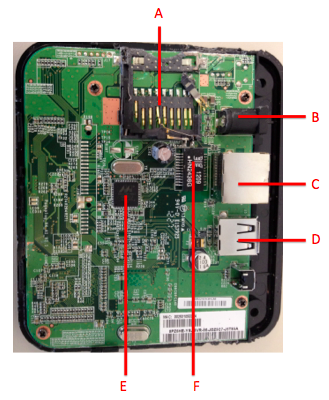
\includegraphics[width=.2\textwidth]{safeplug_listed_top}
%  \label{fig:top}
%}
%\qquad
%\subfloat[][Bottom of the Board inside the Safeplug device.]{
%  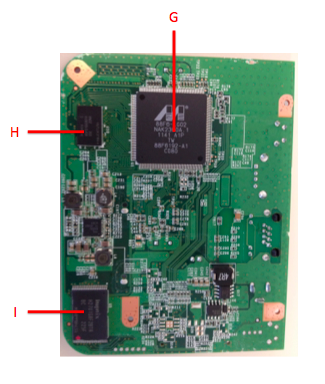
\includegraphics[width=.2\textwidth]{safeplug_hardware_new}
%  \label{fig:bottom}
%}
%\caption{Safeplug circuit board after the teardown.  The explanation of the components is in the text.}
%\label{fig:circuit}
%\end{figure*}

%\begin{figure}[ht]
% \centering
% \subfigure[Top of board.]{
%  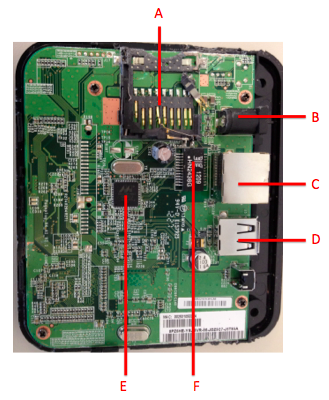
\includegraphics[width=.2\textwidth]{safeplug_listed_top}
%   \label{fig:top}
%   }
% \subfigure[Bottom of board.]{
%  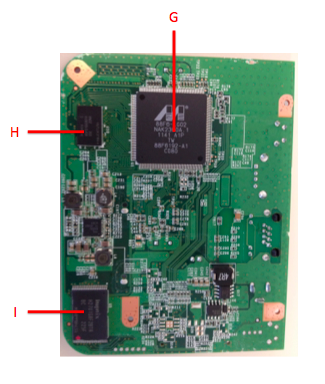
\includegraphics[width=.2\textwidth]{safeplug_hardware_new}
%   \label{fig:bottom}
%   }
% \label{fig:circuit}
% \caption[Safeplug circuit board after the teardown.  The explanation of the components is in the text.]{%
%  Safeplug circuit board after the teardown.  The explanation of the components is in the text.}
%\end{figure}

\subsection{Software on the Safeplug}
\begin{table}[!t]
\renewcommand{\arraystretch}{1.3}
\caption{Software and the corresponding version numbers on the Safeplug as of May 2014.}
\label{versions}
\begin{center}
\small
  \begin{tabular}{|l|c|c|c|}
    \hline
    Safeplug Software & Version & Date & Up To Date\\ \hline
    Linux Kernel & 2.6.31.8 & 2009 & No\\ \hline
    Lighttpd Web Server & 1.4.33 & 2013 & No\\ \hline
    Privoxy Proxy & 3.0.21 & 2013 & Yes\\ \hline
    Tor & 0.2.3.25 & 2012 & No\\ \hline
    Dropbear sshd & v0.52 & 2008 & No\\ \hline
  \end{tabular}
\end{center}
\end{table}

Table \ref{versions} shows the software used by the device, the corresponding version of the software, the date of that version's release, and if it is up to date as of May 2014.  There are many known vulnerabilities in the pieces of software that are not up to date~\cite{cve1, cve2, cve3}.  

%The Safeplug runs version 2.6.31.8 of Arch Linux for ARM, which was produced at the end of 2009.  Unsurprising for its age, there are a number of network vulnerabilities for this version of the kernel - most of which produce denial of service attacks if an adversary sends a particularly formed packet \cite{kernelcve}.  This is the same version of Linux that runs on Version 4 of Pogoplug's Mobile platform \cite{archforum}.  The age of the kernel and the inability to patch the kernel and its libraries creates a large security risk for the Safeplug.  For example, although the Safeplug does not appear to use the recently patched GNUTLS library, if a similar problem had been discovered in one of the Safeplug's libraries, users would have to trust Safeplug to discover and apply the new patch.
%
%As mentioned in the instructions shown in Figure~\ref{fig:instructions}, the Safeplug has an online activation process during which it downloads the software packages it uses to function.  The software installed by the activation process on the Safeplug is in the \verb!/opt/xce! folder of the root filesystem and includes Lighttpd, Privoxy, and Tor.  
%
%Lighttpd is an open-source web-server, which serves the settings page on the device - the project's description mentions ``security, speed, compliance, and flexibility [... while being] designed and optimized for high perfomance environments'' \cite{lighttpd}.  The version of Lighttpd on the box is 1.4.33, which was released on 27 September 2013 and is only one version behind.  The current version of Lighttpd, which has a number of security fixes, was released on 20 January 2014, after the original release of the Safeplug devices.  However, checking for an update from the Safeplug does not lead to any updated software installation.  Privoxy is a ``non-caching web proxy with advanced filtering capabilities for enhancing privacy, modifying webpage data and HTTP headers, controlling access, and removing ads and other obnoxious Internet junk'' and it specifically advertises its ``flexible configuration'' \cite{privoxy}.  Privoxy is also open source.  The version on the device is 3.0.21, which is the most recent release. The version of Tor is v0.2.3.25 from November 2012.  The current stable version of Tor is v0.2.4.20 from December 2013.  Unlike Lighttpd and Privoxy, the Safeplug does not contain the most up-to-date version of Tor from when it was released.
%
%The fourth piece of software the device, which is not installed during the activation process and is in a different location (\verb!/usr/sbin!) is the Dropbear SSH server and client, used to support SSH access to the device \cite{dropbear}.  The Safeplug uses its own configuration files to determine how these pieces of software are set up and used.  The version of Dropbear on the Safeplug is v0.52 from 2008, which is extremely out of date.  Given the different location and installation methods, it seems likely that this was from the older Pogoplug device and is not designed to be updated in the same manner as the rest of the Safeplug software.  However, the SSH server is active and listening on port 22.

This software executes the proxying through Tor and ad-blocking functions via Tor and Privoxy, while the Lighttpd server allows users to modify settings via a JavaScript-generated POST request to a shell script, {\tt xspctrl}, running via CGI.  The CGI handler copies a number of environment variables, and then forks and runs {\tt xspctrl} via {\tt execve} (in the constructed environment). {\tt xspctrl} contains a method for each settings change; these methods execute any necessary Safeplug binary files (go\_update, go\_upgrade, go\_sshd, or go\_updateexceptions) and then return a HTTP response.

%\begin{figure*}
%\centering
%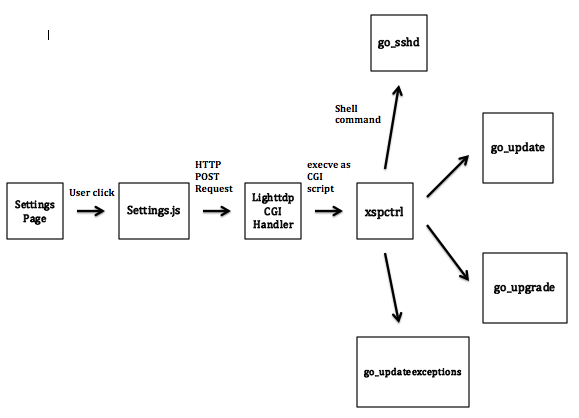
\includegraphics[width=.55\textwidth]{new_callgraph}
%\caption{The call graph for modifying the Safeplug settings page.}
%\label{fig:callgraph}
%\end{figure*} 

%\subsection{Networking}
%The Lighttpd, Privoxy, and Dropbear software give some indication of the networking services on the device.  We used \texttt{nmap} to scan the ports.  Before the activation of the Safeplug, only ports 80 (HTTP) and 3333 (unknown purpose) are open.  After the activation, port 22 for SSH, port 80 for settings access and port 8080 for http-proxy are open.  When Tor is turned on as a relay, port 9001 is opened as well.  This corresponds with the note on the settings page about Tor relays discussed in Section \ref{port9001} below.
    
\subsection{Configuration on the Safeplug}
\label{spconfig}
The Safeplug configuration files can be found in \verb!/opt/xce/etc! and include \verb!sp.conf!, \verb!sp_version!, and \verb!sp_torexceptions!.  The first contains all of the configuration details: whether to use Tor, whether to block ads, and whether to act as a Tor relay or exit relay. The version file is used during the call to check for updates in the \verb!xspctrl! script, and the exceptions file is used by the Privoxy configuation to control the whitelist of sites not to connect to via Tor.  These configuration files are read by the scripts in \verb!/opt/xce/etc/init.d! which enable Lighttpd, Privoxy, and Tor.  As expected, Privoxy looks at the \verb!tor!, \verb!ad-block! and \verb!exceptions! configurations, and Tor reads the \verb!sp.conf! file to determine the correct Tor configuration file (regular, relay, or exit relay).

\section{Usability}
Several aspects of the user experience of the Safeplug also affect the security of the device.

\subsection{Information Prior to Using the Device: Terms of Service}
\label{tos}
The Terms of Service (TOS) are never presented to the user: they aren't presented in the Safeplug package or shown during the activation process, and are only available through a small link at the bottom of the Safeplug website~\cite{safeplug}.  

One of the topics the TOS discusses is the use of open source software.  A standard term of many open source licenses states that a company that uses the open source software must list the software used and its license, as well as the open source code of their own software that uses the license.  The TOS contains a link to a page that would supposedly comply with this requirement: \url{http://pogoplug.com/home-en-developers-open-source.html}, but the link is dead; instead, the reader sees a 404 error \cite{safeplug}.  There is an open source page at \url{http://pogoplug.com/opensource}, which describes several pieces of software used by the Safeplug; however, there is no way to find this page from the Terms of Service or the Safeplug website.

\subsection{Activation and Setup}
%The first step was to plug Safeplug into our router and activate our device.  We followed the simple instructions, activated our device, and then ended on the configurations page.  The configurations page shows a variety of platforms and browsers, shown in Table \ref{table_example}, and links to proxy configuration instructions for each one.  For every browser on every client device that the user wants to protect, they must set up the Safeplug as the browser's HTTP proxy and ensure that the proxy stays set up when the browser is updated or re-installed.

First, we activated the device by following simple instructions.  Next, we followed the configuration instructions based on our specific platform and browser (the options are shown in Table \ref{table_example}) to set up the Safeplug as our browser's HTTP proxy.  The last step was to modify the settings; this page is shown in Figure~\ref{fig:settings}.  We can turn Tor on/off, turn ad-blocking on/off, and turn Tor relay node ability on/off (and if on, an additional option appeared to allow the device to be an exit relay).  Additionally, we can specify ``white-listed'' domains that will be connected to directly even if Tor is turned on, without going through the Tor network.

\begin{table}[!t]
\renewcommand{\arraystretch}{1.3}
\centering
\small
	\begin{tabular}{|c|c|}
	\hline
		Platform & Browsers \\ \hline
		Windows	& Internet Explorer, Chrome, Firefox \\ \hline
		OSX & Safari, Chrome, Firefox \\ \hline
		iOS	& Safari \\ \hline
		Android	& Chrome \\ \hline
	\end{tabular}
\caption{The platforms and browsers that the Safeplug settings page provides instructions for.}
\label{table_example}
\end{table}



\begin{figure}
  \centering
  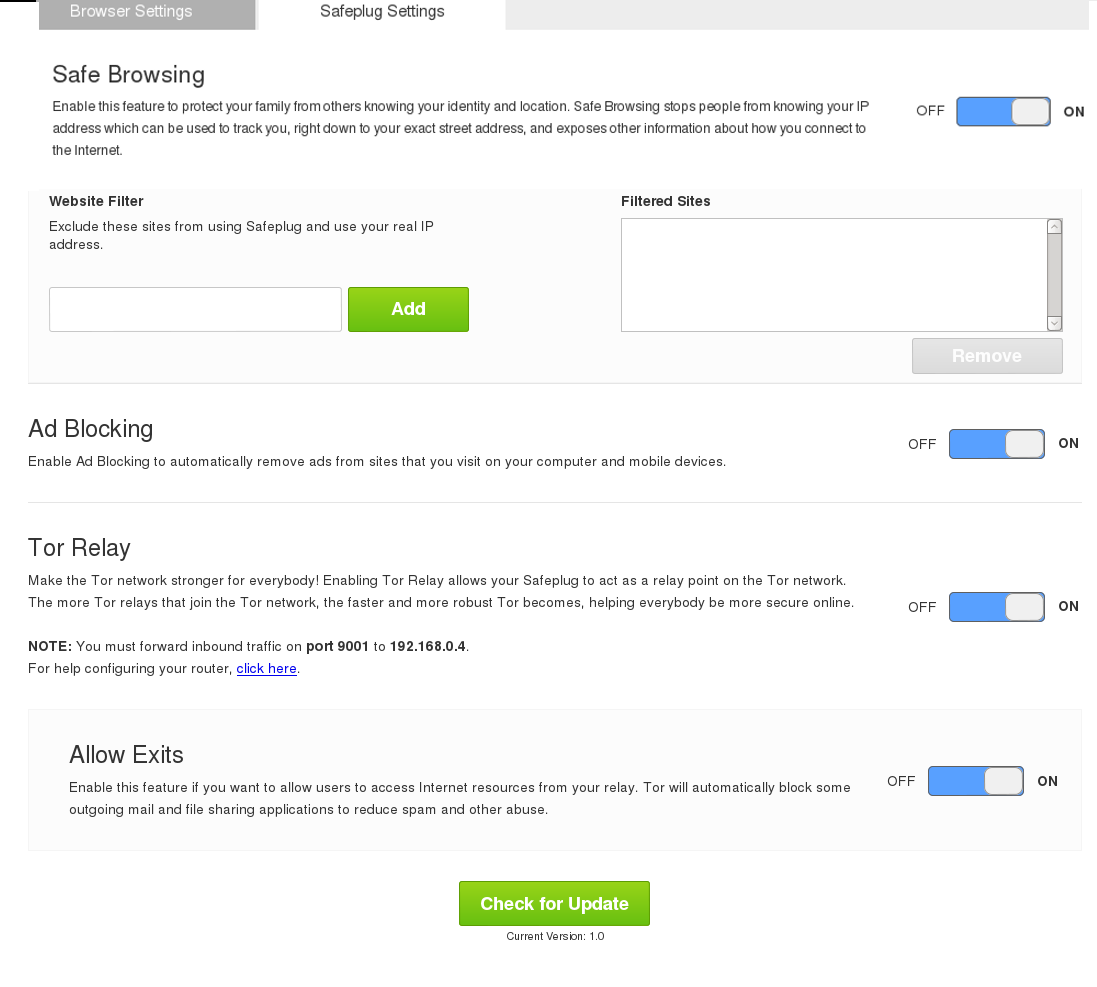
\includegraphics[width=.5\textwidth]{settings_with_exit}
  \caption{Safeplug settings page.  The last button ``Allow Exits'' only appears if the relay option above has been turned on.}
  \label{fig:settings}
\end{figure}

%\subsection{Explanation of Tor Configuration Options}
%\label{port9001}

%The settings page describes Tor in an extremely basic way:

%\begin{quotation}
%``Safeplug uses the Tor network to secure your Internet connection.  Tor works by routing your Internet through a series of random destinations, much like driving a twisty, complicated route to throw off someone who is following you, making it impossible for websites and organizations to identify the source or destination of Internet traffic.''
%\end{quotation}

%On the other hand, it assumes a much higher level of knowledge about networks for users trying to configure a relay:
%\begin{quotation}
%You must forward inbound traffic on port 9001 to [IP-of-Safeplug]. For help configuring your router, click here.''
%\end{quotation}

%The link provided is to an advertisement-filled and confusing website.

It is important to note that there is no explanation of relay or exit nodes.  Using Safeplug as an exit node has possible legal repercussions.  As an exit relay, all traffic that exits the node can be traced back to the Safeplug's IP address; it is likely that some of this traffic contains illegal information or is part of illicit activities.  The Tor Project recommends not running an exit relay from a user's home.  Considering that the Safeplug is intended for home use, it is a poor design choice to allow the user to use it as an exit relay without providing the user with any contextual information.

%\subsection{Internet Use}
%\label{inetuse}

%\begin{figure*}[tb]
%\centering
%\subfloat[][Web page before using Tor and ad-blocking.]{
%  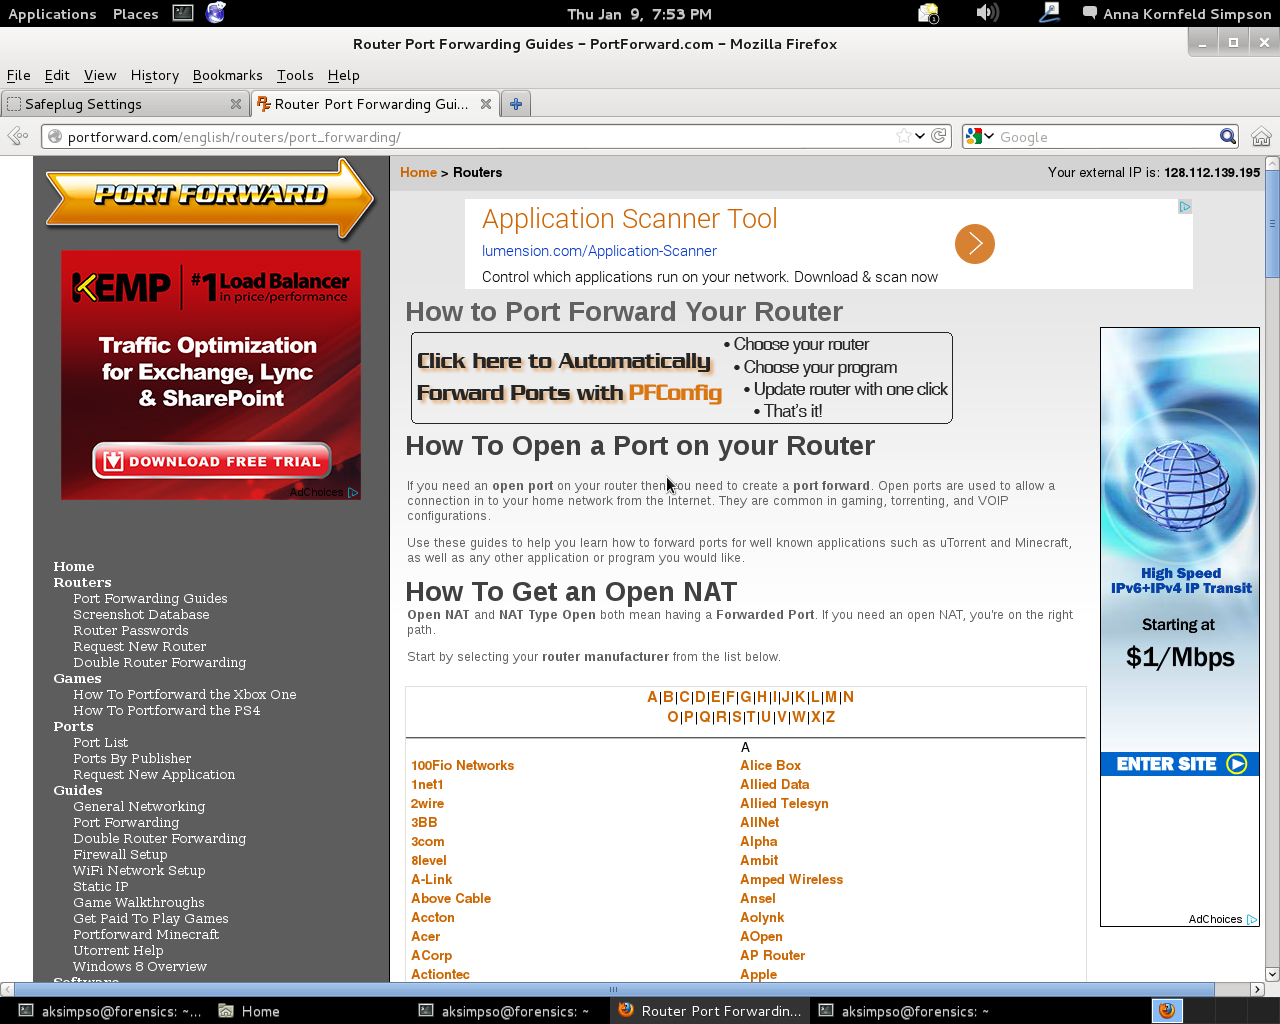
\includegraphics[width=.3\textwidth]{before}
%  \label{fig:before}
%}
%\quad
%\subfloat[][Web page after using Tor and ad-blocking.]{
%  
\includegraphics[width=.3\textwidth]{after}
%  \label{fig:after}
%}
%\caption{Application of Safeplug proxy settings.}
%\end{figure*}

%Next, we examined popular webpages, with an eye for changes in the user experience.  A user would probably decide not to use Safeplug if they could not read their web pages (due to a different language), or if they could not log into their accounts (some web sites will lock a user out if they try to log in from multiple countries in a short time period).  While browsing the Internet, we experienced some pages in German and Swedish; if a user is not familiar with Tor, they may not understand why this is happening.  We were also prompted with a request to ``Enter the name of the city where you usually sign in'' when we tried to log into our Google account, indicating that Google noticed we were trying to login from an ``unusual'' location.

\subsection{Cookies}  
While browsing the Internet in a fresh browser session, we used FourthParty, a plugin developed by Jonathan Mayer to collect information about cookies and other browsing data, to confirm the presence of first-party cookies~\cite{fourthparty, mayer2012third}.  More interesting and damaging to the user's control over their anonymity would be third-party cookies because the user cannot remove those just by logging out.  Most browsers require a trip to the browser settings to clear cookies (or not have them set in the first place).  When collecting data on the existence of third-party cookies, we analyzed two separate browsing sessions; they were both new sessions with no cookies.  One of the sessions used the ad-block feature of the Safeplug and the other did not.  We found many third-party cookies in both sessions; these included cookies from: abmr.net, bizographics.com, krxd.net, and bluekai.com among many others.  The ad-block functionality on the Safeplug reduced, but did not eliminate, these third-party cookies.

Although Safeplug has a warning about clearing cookies on their FAQ page, it only mentions clearing cookies after a browser session.  This does not prevent the tracking of a user during their browser session from website to website; preventing this requires knowledge and vigilance from the user, or a browser that does not accept third-party cookies, such as the one provided in the Tor Browser Bundle.

\subsection{Browser Fingerprinting}
We used Panopticlick~\cite{panopticlick} to examine the fingerprint of a freshly installed Firefox browser running through the Safeplug proxy.  Panopticlick found the browser to be unique, which means that websites that did fingerprinting could very accurately track, correlate, and de-anonymize user traffic without knowing the IP address or even storing a cookie.  The presence of the Safeplug, as an HTTP proxy, should be completely undetectable by the fingerprinting service because HTTP is designed to make proxies transparent.  Unlike the Tor Browser, Safeplug users do not have the fingerprints of other users of the service to help hide their fingerprints.  Allowing the user to use their own browsers significantly increases the amount of variation and customization between users and therefore the likelihood of having a unique fingerprint.

\subsection{Latency}
If the latency of web requests using the Safeplug is noticeably longer than that of normal Internet use, users may be deterred from using the device.  Similarly, if turning Tor on adds a significant time delay, the user may only turn on the ad-blocking feature (without Tor).  We recorded the time for a web request on the following settings:

\begin{itemize} %\setlength{\itemsep}{2mm}
\item Plain Firefox (no use of the Safeplug device)
\item Firefox, no Tor, no ad-blocking (traffic running through the Safeplug device)
\item Firefox, Tor, no ad-blocking (using the Safeplug device)
\item Firefox, Tor, ad-blocking (using the Safeplug device)
\item Firefox, no Tor, ad-blocking (using the Safeplug device)
\item Tor Browser Bundle with Safeplug (all settings off)
\item Tor Browser Bundle (no use of the Safeplug device)
\end{itemize}

For each of the settings, we took 20 measurements because we were confident this would give us enough data points that would span multiple Tor circuits; Figure~\ref{fig:latency2} shows the average time of a web request on each of the specified settings for three different web pages.  When taking these measurements, we loaded the page, but did not scroll; in many cases more objects are loaded when scrolling down a page.  The differences between web pages can most likely be attributed to the amount of advertisements and content running in plugins (such as video) on the web page.  

\begin{figure}
  \centering
  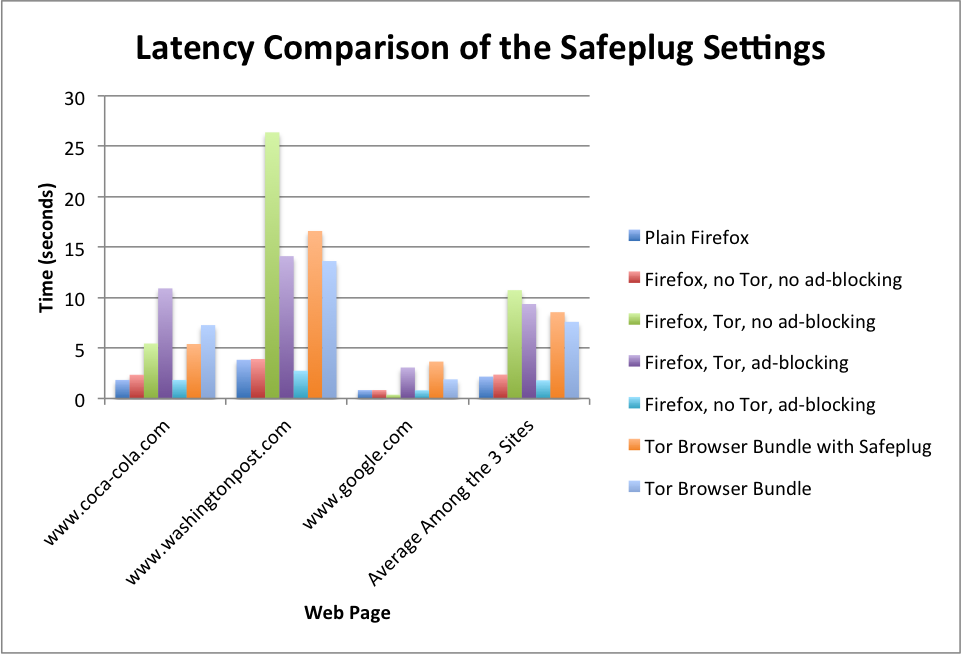
\includegraphics[width=0.5\textwidth]{latencygraph}
  \caption{Latency of web requests.}
  \label{fig:latency2}
\end{figure}

The average web request time for accessing \url{www.washingtonpost.com} is greatest on the same settings that the average web request time for \url{www.google.com} is the least. This setting did not include ad-blocking, and therefore \url{www.washingtonpost.com} had to render each ad (which it requested through Tor); \url{www.google.com} does not have any ads.

\begin{figure}
  \centering
  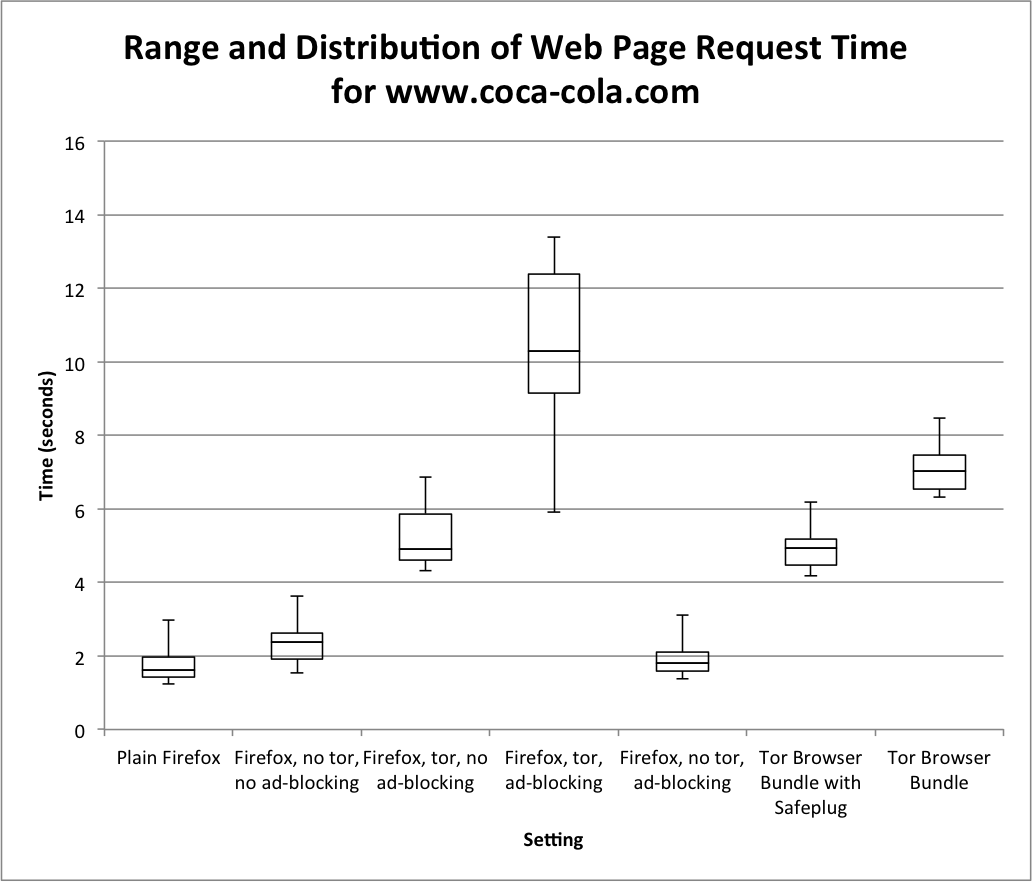
\includegraphics[width=0.5\textwidth]{rangeanddistcocacola}
  \caption{Web request time variation for www.coca-cola.com.}
  \label{fig:boxandwhisker}
\end{figure}

Figure~\ref{fig:boxandwhisker} displays the variation among fetch requests for each setting when fetching \url{www.coca-cola.com}.  Despite performing these fetches close in time, the greater variation for settings using Tor shows that more than one Tor circuit was used, and therefore, we were not simply measuring the variation in Tor circuit performance.  

The latency of using the Safeplug with Firefox, Tor, and ad-blocking is comparable to that of using the Tor Browser Bundle.  For all three web pages, the Tor Browser Bundle had slightly lower latency; the Tor Browser Bundle blocks scripts, and for web pages such as \url{www.coca-cola.com}, this provides a significant latency decrease and better protects privacy.  This, in conjunction with the fact that the Tor Browser Bundle is free and is issued directly from The Tor Project, shows a convincing argument to use the Tor Browser Bundle in place of the Safeplug.  

\section{Privoxy vs. Tor Browser Bundle}
The Safeplug uses two primary technologies: Tor and Privoxy.  The Tor Project has developed the Tor Browser Bundle (TBB), which is a free custom browser that uses Tor as well as other protection mechanisms to help preserve a user's privacy.  A differentiating factor between the Safeplug and the TBB is the use of Privoxy; in order to determine the effectiveness of the Safeplug in comparison to that of the TBB, we must measure the value of Privoxy against the other features of the TBB.  We ran a privacy study on the use of Firefox, Firefox with Privoxy, and the TBB; our data was collected by running crawls on the Alexa Top 100 sites in each of the specified browsers~\cite{alexa}.  All browser configurations were modified with Pagestats \cite{pagestats} and Cookie Manager+ \cite{cookiemonster} to aggregate information about third party requests, JavaScript objects, flash objects, and third party cookies.  Because measuring privacy is a difficult task, we measured potential ways for a user's privacy to be compromised.  First, we recorded how many third party domains were accessed total (throughout the crawl); in addition, we recorded the total number of JavaScript and Flash objects received from third parties, as well as the total number of third party cookies received.  We then found the on-average, per-page numbers corresponding to these measurements by dividing the totals by 100.  These fractions are shown in Table~\ref{tbb}.

\begin{table}[!t]
\renewcommand{\arraystretch}{1.3}
\centering
\small
	\begin{tabular}{| p{1.85cm} | p{1.3cm} | p{1.25cm} | p{.7cm} | p{1cm} |}
	\hline
		Configuration & Third Party Domains & Third Party JavaScript & Third Party Flash & Third Party Cookies \\ \hline
		Plain Firefox	& 0.64 & 0.01 & 0.01 & 0.88 \\ \hline
		Privoxy & 0.72 & 0.00 & 0.01 & 0.84 \\ \hline
		Tor Browser	& 0.58 & 0.01 & 0.00 & 0.00 \\ \hline
	\end{tabular}
\caption{Measurements of using Firefox, Privoxy, or the Tor Browser Bundle; the numbers represent the average number of Third Party Domains accessed per page, the average number of Javascript objects received from third parties per page, the average number of Flash objects received from third parties per page, and the average number of third party cookies received per page.}
\label{tbb}
\end{table}

It is clear that the Tor Browser Bundle performed the best in most categories. The one category where Privoxy performed better than the Tor Browser Bundle is in the number of JavaScript objects received from third parties; this can be attributed to the fact that our measurements were taken using the default settings for the Tor Browser Bundle, which allows JavaScript~\cite{torproject}.  This is explained on the Tor Project's website; they explain that disabling JavaScript causes some web pages to break, making the browser less user-friendly.  The user has the option to disable JavaScript by simply clicking a button.  This shows that the Tor Browser is a less expensive alternative to the Safeplug, and provides more privacy protections.    

\section{Vulnerabilities}
As we discovered during our software analysis, the Safeplug has a remote procedure call (RPC) capability.  This is a script called \verb!xspctrl! found in \verb!/opt/xce/html/svc!.  Functional calls to this script include the ability to enable and disable all of the Safeplug settings, including Tor, ad block, and Tor relay.  None of them require any authentication.

\begin{figure}
  \centering
  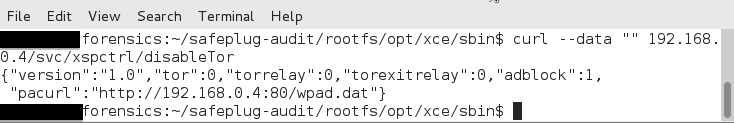
\includegraphics[width=.5\textwidth]{disabletor2}
  \caption{Disabling Tor as an RPC attack.}
  \label{disable}
\end{figure}

\subsection{Insider Attack}
The Safeplug has no validation or authentication on the settings page for these RPC calls, so any malicious party inside the home network can easily modify the settings.  Unlike many home routers that use a similar system for settings modification, there is no username/password combination necessary to access the settings page.  A more technically advanced user could send the call directly to the RPC server.  Figure \ref{disable} shows an example of the RPC version of this attack.  If the adversary can get into the network they can perform these attacks.  For example, if the user has an open WiFi network, then anyone nearby can launch this attack - potentially peforming a sort of drive-by deanonymization. 

Since the RPC version of the attack just involves basic Internet tools (the ability to send a POST request), the attacker could also be any kind of device on the local network, or the local gateway itself, if it is compromised.

\subsection{CSRF Attack}
Any external website can also perform the above attack by returning a correctly formatted POST string via an internal user's browser.  This executes the same functionality as the Insider Attack, but the attacker does not need to be on the local network.  This Cross Site Request Forgery (CSRF) attack requires a nonmalicious insider user to visit a web page controlled by the attacker, allowing the attacker to send the POST to the Safeplug.  If the attacker does not know the IP address of the Safeplug, he can perform an exhaustive search on the address space.  We implemented this attack with less than 20 lines of JavaScript code.  The following steps are necessary for the attack:

\begin{enumerate} \setlength{\itemsep}{.2mm}
\item Set up a web page with the JavaScript code, which will send the POST request of the following format to all addresses in the common ranges: \url{http://<IP address>/svc/xspctrl/disableTor}.
\item Send the malicious link to a user in the targeted private network.
\item Once the user clicks the link and loads the malicious site, the correctly formatted POST request will be sent to every IP address in the ranges.  
\item Tor is disabled silently.  The user must check or refresh her Safeplug settings page to learn that Tor is off.  
\end{enumerate}  

While this attack requires a greater amount of time because the local IP address of the Safeplug must be guessed via search, the number of private address spaces is small, and the space likely to be occupied by a Safeplug on a home network is even smaller.  

The largest observed time to send requests to the 192.168.0.0/24 space was approximately 400 milliseconds; the entire attack costs approximately 800 milliseconds for sending requests to both 192.168.0.0/24 and 192.168.1.0/24 ranges - even when the website was being loaded over Tor.  In the case of a private network in the range of 172.16.0.0/16, the attack took less than 12 minutes (this generates script timeout warnings in most major browsers, which affects the timing of this attack).  This means that it would take a few hours to send requests to the full 172.16.0.0/12 range, which is commonly used in business networks.  The final private network space is 10.0.0.0/8 which is too large for an exhaustive search, but some simple optimization might make it feasible as well.  For example, using a GET request to get and parse the Safeplug settings page would allow the script to positively identify the Safeplug and stop the search.  However, the 192.168.0.0/24 and 192.168.1.0/24 ranges are much more common in home networks; because Safeplug is geared towards home network use, in most cases the script will take less than a second.

In addition to disabling Tor, the attacker can modify any other settings on the device.  This includes: enabling/disabling Tor, enabling/disabling ad-blocking, enabling/disabling the use of the device as a Tor relay node [note: enabling requires the user to do additional setup], enabling/disabling the use of the device as an exit node (if it is already a relay).  Lastly, the attacker can also modify the user's whitelist of sites that should not be routed through Tor.  This whitelist attack is particularly dangerous because the change is silent and much harder for the user to notice the addition of a single website to the whitelist than a global loss of Tor.

\subsection{Gaining Access through SSH}
\label{sec:SSH}
    Another command available to the RPC server is enabling SSH to the device.  SSH instructions for Pogoplug's other device (called Pogoplug) are widely available online and an email in the Tor-talk mailing list confirmed the instructions are the same for the Safeplug \cite{ceadmin}:
%\begin{lstlisting}
%curl --data ``'' http://<IP>/svc/xspctrl/enableSSHD
%ssh root@<IP-of-Safeplug>
%password: ceadmin
%\end{lstlisting}

{\tt \small
\begin{verbatim}
curl --data ``'' http://<IP>/svc/xspctrl/enableSSHD
ssh root@<IP-of-Safeplug>
password: ceadmin
\end{verbatim}
}

Having a publicly available root password means that SSH is done effectively without authentication.  Once the box was activated and had Lighttpd installed, the SSH procedure was available and any adversary on the home network could log into the box and install malware, surveillance software, or virtually anything they desired.

\subsection{Spoofing the Installation Server}
\label{dnsspoof}
An additional dangerous class of vulnerabilities comes from the lack of HTTPS during the initial installation process.  We discovered that the script that performs this installation is downloaded via TCP from an IP address provided by the Pogoplug servers.  This script (run as root) then downloads the Safeplug's software (Tor, Privoxy, Lighttpd, and wget) and checks it against MD5 hashes provided in the script, but we could not find any signs of verification of the script itself.  An adversary could use DNS spoofing or compromise the Pogoplug server and force users to download a malicious script - for example, something that turns the Safeplug into a surveillance box while appearing to provide the correct functionality.  Because the activation occurs over TCP in the clear, an adversary who can spoof DNS replies to the user can install arbitrary software onto the Safeplug box.  This turns a device that does not live up to expectations, but is otherwise harmless, into something that actively harms security on the network.  We were unable to observe a post-installation update from Pogoplug due to none being provided to users in the 6+ months since the Safeplug was released, but examining the update scripts on the Safeplug indicates that this update process occurs over HTTPS, so that only the initial download during device activation is vulnerable. However, DNS spoofing would still defeat the authentication of update binaries provided by HTTPS. In short, Pogoplug should be signing both the code used in updates and the code downloaded during the initial installation with a key whose corresponding verification key is part of the device's factory image. Pogoplug already provides several certificates in the factory image to establish roots of trust, so it would be a minimal engineering effort to include their own update-signing certificate.\footnote{N.B. There could be such a certificate already on the device that we haven't found. Because there have been no updates, we cannot determine whether signatures are present on the update code. We hypothesize that they would not be present, based on the fact that they were not present in the downloads for device initiation.}

\section{Related Work}
To our knowledge, there has been no other study analyzing the security of Pogoplug's Safeplug device.  However, there has been much prior research on Tor~\cite{tor} and fingerprinting.

{\bf Tor.} Prior security evaluations of the Tor network reveal a myriad of potential vulnerabilities.  A significant area of research on Tor relates to diversity of autonomous systems (ASes).  Researchers argue that a user's anonymity may be compromised by using geographically diverse ASes~\cite{feamster, murdoch2}.  There has also been proven traffic correlation attacks that are efficient on the Tor network~\cite{murdoch, overlier}.  Johnson, Wacek, Jansen, Sherr, and Syverson found that in a period of six months, 80\% of all users may be deanonymized by a reasonably realistic Tor-relay adversary~\cite{tor2}.  While Safeplug does not introduce or modify how Tor is used, it routes all traffic through the Tor network; Safeplug is also vulnerable to the attacks found in prior research on Tor.  

{\bf Fingerprinting.}  Website fingerprinting attacks as well as remote physical device fingerprinting attacks have shown they can identify users, even when specific defenses have been used in order to prevent them. Previous research has shown that web page fingerprinting attacks are possible~\cite{dyer, herrmann, panchenko}.  Cai, Zhang, Joshi, and Johnson found that their fingerprinting attack is successful 83.7\% of the time when the defense is the use of Tor~\cite{fingerprint1}.  These results can be extended to the security of Safeplug.  Because Safeplug uses Tor to anonymize users, it may be susceptible to fingerprinting attacks.

\section{Discussion}
\subsection{Necessary Fixes}
The most critical engineering fix is authentication in the POST calls to prevent the CSRF attack.  A typical approach to preventing CSRF attacks is using a cookie and a hidden form field set in the settings page of the Safeplug hosts; the cookie must be returned by the browser when making the POST request to the RPC server \cite{csrfdef}.  Although someone doing a CSRF attack such as the one described above could get the cookie sent, because of the same-origin policy, the adversary would not be able to examine the contents of the cookie to determine what to put in the form field. Pogoplug should also take steps to secure

\subsection{Structural Problems}
However, there are much more significant structural problems with implementing a Tor connection via an HTTP proxy.  Several of the usability problems involve user awareness and vigilance.  For example, cookies and fingerprinting problems mean that users could still be tracked across websites, regardless of whether the ad-block functionality on the Safeplug is enabled.  

One type of client that deserves special attention is a mobile phone user.  Although the Tor Project publishes an Android app called Orbot on the Android Market, which is supported for Android versions 2.3 and later, there are no official Tor apps for iPhones or other non-Android devices~\cite{orbot,amorbot}.  Safeplug provides proxy functionality and instructions for Safari on the iPhone and Chrome on Android.  However, while this does supposedly give the option for more mobile users to make use of Tor, proxy configuation on mobile devices comes with significant usability issues.  For example, proxying would only work while the user is on the same wifi network as the Safeplug.  If any data is sent over the cellular network or another wifi network, then the security of Tor is lost.  Additionally, the user may have to disable the proxy whenever they move to a different network, and remember to re-enable it when they want to use Tor.  This is certainly not transparent usability.  Users who are truly concerned about anonymity online should eschew the Safeplug and purchase a device that supports the Tor Browser Bundle or other Tor Project software.

\subsection{Opportunities}
Despite all the structural problems, is there a market for a Torifying piece of hardware?  Given the security and privacy pitfalls in comparison to a piece of software such as the Tor Browser Bundle, there seems to be no reason for a user who can run the Tor Browser Bundle to purchase the Safeplug or any other device.  For mobile phones, the proxy problems with mobility contribute to an already high usability cost.  However, there are an emerging class of ``smart home'' devices which may connect to the Internet.  It is possible that some of these devices can be configured to use an HTTP proxy or some other middle box to Torify their traffic to an external service provider.  For them, is the benefit of some anonymity via a Safeplug-like device worthwhile?  Since the data sent by these devices to the service provider likely contains identifying information, the use of Tor would only protect the user's location at the expense of connection time and load on the Tor network.  Since proxy configuration on such devices is likely to be difficult and the amount of information hidden is unlikely to be worth the effort, a Torifying box that functions as a proxy is of questionable value in this space as well.

\section{Future Work}
A more in-depth analysis of the performance of the Safeplug would be useful in the future.  The performance of the Safeplug reflects its usability, and would be helpful in determining the trade-offs of using the device.  Additionally, clearer privacy metrics are needed to help evaluate privacy-enhancing technologies, such as the Safeplug.  

\section{Conclusion}
Ultimately, the structural concerns of the Safeplug ``Torifying proxy-in-a-box'' strategy indicate that this is problematic as a method for security and anonymity online.  It is critical for Safeplug to correct their security errors, particularly the vulnerability to silently disable Tor, in order to protect customers who have already made use of the device, but users who are truly concerned about safety and anonymity online would be better served by the Tor Browser Bundle.

{\footnotesize \bibliographystyle{acm}
\bibliography{paper}}

%\theendnotes

\end{document}







